\documentclass[11pt,letter,nocenter]{revtex4-1}
\usepackage[utf8x]{inputenc}
\usepackage{graphicx}
\usepackage{amssymb}
\usepackage{epstopdf}
\usepackage{mystyle}
\usepackage{amsmath}
\usepackage{bm}

%\setlength\parindent{0pt}

\begin{document}

\title{Estimating quantum mechanical effects of atomic solids using quantum molecular dynamics with dissipation}
\author{Bing Gu, Robert J. Hinde, Sophya Garashchuk, Vitaly Rassolov}
\affiliation{Department of Chemistry and Biochemistry, Univerisity of South Carolina, Columbia}

\begin{abstract}
 Solid helium-4 is a well-known quantum atomic solid, characterized by large zero-point energy that cannot be described by harmonic approximation. In this paper, we describe  how to use a quantum molecular dynamics method with friction to compute zero-point energy and pair distribution function for large-scale quantum system and use it for solid helium-4 with $180$ atoms.  A new approximation is made for the quantum potential to fix the unbalance problem we encountered while applying linearized quantum force \cite{Garashchuk2004} to systems with large anharmonicity.  It  is shown that the modified fitting procedure is capable of capturing the zero-point energy caused by large anharmonicity. Pair distribution function is also computed at various atomic mass to study the dependence on atomic mass. 

\end{abstract}

\maketitle

\section{Introduction}

 Solid helium-4 is a well-known quantum atomic solid, characterized by large zero-point energy that cannot be described by harmonic approximation, which is a normal way to get an estimate of zero-point energy.  
We will describe how to use a quantum molecular dynamics method with friction to compute zero-point energy and pair distribution function for large-scale quantum system and use it for solid helium-4 with $180$ atoms. 

In the simulation of quantum molecular dynamics, the so-called quantum potential, which requires the amplitude of the whole wavefunction, has to be approximated. In our previous work \cite{Garashchuk2011}, a global linear basis fitting to non-classical momentum  \cite{Garashchuk2004} is used. We encounter an unbalance problem while applying this approach to systems characterized by large anharmonicity.  
 
A new approximation for the quantum potential  is proposed to fix this problem. It is shown that the modified fitting procedure is capable of capturing the zero-point energy caused by large anharmonicity. 
Pair distribution function (PDF) measures the disorder of quantum system. For a classical solid at absolute zero, it is simply some peaks of infinity intensity at values corresponding the pair distances in the system. Due to large zero-point energy, the peaks will be broadened as the wavefunction of the system spreads over space. We study the influence of mass on the pair distribution function.  
% PDF for solid helium-4 is computed at various atomic mass to see the change of PDF due to change of mass. 

Quantum molecular dynamics with dissipation basically describes the interaction of a quantum system with the the environmental degrees of freedom. 
Inclusion of friction directly into the \se may be viewed as a simple way to mimic the effect of energy transfer from the system to the environment while containing quantum dynamics calculations to the system degrees of freedom. In classical mechanics, the frictional force, often considered for processes  happened in condensed phase, is always taken as linearly dependent on particle velocity. The equations of motion for a particle with  position $x$ and momentum $p$ while a friction force exists are as follows, 
\be \dot{p} =-\grad V(x)-\gamma p , ~~\dot{x}  = \frac{p}{m}. \ee
 
The classical trajectory evolves under the influence of an external potential $V( x)$, which is a function of the Cartesian coordinate, $x$, parameter $\gamma$ denotes the friction coefficient. In standard quantum mechanics, the conception of particles is missing, instead wavefunction is use to represent a system. 
However, in de Broglie-Bohm formulation of quantum mechanics, the wavefunction is represented by an ensemble of quantum trajectories. We will extend the idea of friction into dynamics of quantum trajectories, resulting in similar equations of motion except the quantum potential, which includes all the quantum effects. 

This paper is organized as follows. Section \ref{sec:theory} describes the quantum molecular dynamics theory and how to incorporate friction into dynamics. Some details about how to set up the system of solid helium-4 and how to apply the periodic boundary condition is shown in section \ref{sec:sys}. The last section shows the results of simulation, including the computation for zero-point energy and pair distribution function with different atomic mass. 

\section{Formulation}
\label{sec:theory}
\subsection{Bohmian mechanics} 

About the notations used in this paper, without specified, we will use small Arabic letters $(i,j,k...)$ to label trajectories and Greek letters to label degree of freedom (DoF) and bold small letters for vectors and bold capital letters for matrix. Atomic units is used by default.  

In de Broglie-Bohm theory, the wavefunction is represented in polar form with the amplitude $A(\bm x,t)$ and phase $S(\bm x,t)$, which are both real functions of $\bm x$ and $t$, 

\be \psi(\bm{x},t) = A(\bm{x},t) \exp{\left( \frac {\imath}{\hbar} S(\bm{x},t) \right)} \label{eq:polar}. \ee

The probability density is 
\be \rho(\bm{x},t)=\psi^{*}(\bm{x},t)\psi(\bm{x},t)=A^2(\bm{x},t). \label{density} \ee 

Substituting Eq. (\ref{eq:polar}) into TDSE, one obtains
\begin{flalign}
\frac{\partial S(\bm x,t)}{\partial t} &=\frac{\grad S(\bm x,t)^2}{2m}-V(\bm x)-U(\bm x,t), \label{eq:qhje} \\ 
\frac{\pa \rho(\bm x,t)}{\pa t} &=-\grad \left( \rho(\bm x,t) \frac{\bm{\grad}S}{m} \right)  \label{eq:density}, \\
%\frac{\partial A^2(\bm x,t)}{\partial t} &= -\bm \grad \left [ A^2(\bm x,t)\cdot \frac{1}{m} {\bm \grad S(\bm x,t)}\right ] \label{eq:pair1}, \\
\end{flalign}
where 
\be U(\bm{x},t) = -\frac {\hbar^2}{2m} \frac {\nabla^2 A(\bm{x},t)}{A(\bm{x},t)}. \label{eq:qp}. \ee
%Full derivative ot time $t$ is defined as
%\be \frac{d}{dt} = \frac{\partial}{\partial t}+ \bm{v}\nabla. \ee 
$U(\bm x,t)$ is  the so-called non-local time-dependent quantum potential, and is proportional to $\hbar^2$. 
Without loss of generality, we assume the mass $m$ is the same for each DoF. If not, we can simply use a diagonal matrix $\bf M,   $ to replace $m$, where 
 \be m_{ii} =m_i, i \in [1,N_{dim}] \ee, 
$N_{dim}$ is the number of DoF.  
% It is important to note that the polar form is not useful at nodes, where $\psi=0$. The phase is well-defined for times before and after the node passes over a fixed point in space, not at the instant that the node crosses the point.

%The probability flux associated with $\psi(\bm x,t)$ is given by
%\be j(x,t)=\frac{\hbar}{2m\imath}\left [ \psi^*(x,t)\frac{\partial \psi(x,t)}{\partial x}-\psi(x,t)\frac{\partial \psi^{*}(x,t)}{\partial x} \right ]. \label{eq:flux} \ee 
%This quantity gives the rate at which probability flows past a fixed point. if we insert the polar form of the wave function into equation \ref{eq:flux}, we get the flux in terms of the density and the derivative of the action
%\be j(x,t)=\rho(x,t)\cdot \frac{1}{m}\frac{\partial S(x,t)}{\partial x}. \ee
%In classical fluid flow, the flux is given by $j(x,t)=\rho(x,t)v(x,t)$, where $v(x,t)$ is the flow velocity of the fluid. 
%In equation \ref{eq:flux}, we will make this association and refer to the flow velocity of the probability fluid as the function \cite{wyatt2005}

%Equate \be v(x,t) = \frac{1}{m}\frac{\partial S(x,t)}{\partial x}. \ee
%Returning to equation \ref{eq:pair1}, the term in brackets in the right side is just the probability flux, thus, we finally obtain the standard form of the continuity equation
%\be \frac{\rho(x,t)}{\partial t} = -\frac{\partial j(x,t)}{\partial x} = -\frac{\partial}{\partial x}\left [ \rho(x,t)v(x,t) \right]. \ee
%The three-dimensional form of this equation in the Eulerian picture is given by 
%\be \frac{\partial \rho(\vec{r},t)}{\partial t}=-\vec{\grad}\cdot \vec{j}(\vec{r},t)=-\vec{\grad} \cdot \left [ \rho(\vec{r}, t)v(\vec{r},t) \right ]. \label{eq:3dflux}\ee

% quantum Hamiltion-Jacobi equation

Eq. (\ref{eq:qhje}) is the Eulerian version of the \textit{quantum Hamiltion-Jacobi equation}, differing from classical \textit{Hamilton-Jacobi equation} by the quantum potential term. 
The wavefunction can be discretized in coordinate space by quantum trajectories (QTs) with position $\bm{x}$ and momentum $\bm{p}$, defined as 
\be {\bm p}=\bm \grad S, \label{eq:p} \ee
where $\bm \grad$ here represents a column vector of differential operator, 
\be \bm \grad = \left[ \begin{array}{c}   \pa_{x_1} \\ \pa_{x_2} \\ \vdots \\ \pa_{x_{N_{dim}}}  \end{array} \right] \ee 
When $\hbar \rightarrow 0$, $U$ becomes negligible and all of the trajectories become independent of each other, which is the classical limit. 
The quantum potential $U$ can be considered as a nonclassical contribution to the kinetic energy. 
Trajectories from an quantum ensemble, representing the wavefunction, are assigned certain weights $w_i$, that depends on the initial probability density  and the volume associated with each trajectory,  
\be w_i = \psi^*(\bm x_i,t_0)\psi(\bm x_i,t_0) d \bm x_i(t_0) = A^2(\bm x_i,t_0) d \bm x_i(t_0) \label{eq:weights} = \rho(\bm x_i,t_0)d \bm x_i(t_0). \ee
Space of non-negligible density is sufficiently sampled with trajectories, $N_{traj}$ is the number of trajectories,
\be \sum_{i}^{N_{traj}} w_i \approx \int_{-\infty}^{+\infty} \psi^{*}(\bm{x},t) \psi(\bm{x},t) d \bm{x} = 1 \label{eq:normal},\ee and their weights remain constant in the course of dynamics \cite{Garashchuk2004} in the Lagrangian frame-of-reference, 
\be \frac{dw_i}{dt} = 0.\ee
\noindent
The Lagrangian and Eulerian frame-of-references are connected by 
\be \frac{d}{dt} = \frac{\pa }{\pa t } + \frac{\bm p^T}{m}\bm \grad \ee 
The evolution of trajectories is given by Hamilton's equations of motion,
\begin{flalign} \frac {d\bm x_i}{dt} &= \frac {\bm p_i}{m} , \label{eq:motion1} \\
 \frac {d\bm p_i}{dt} &= - {\bm \grad} \left.(V + U)\right|_{\bm x=\bm x_i} \label{eq:motion2}.\end{flalign}
Here subscript $i$ labels the trajectories. The phase of wavefunction, $S(\bm x_i,t)$, is equal to  the  action function $S_i$ of each trajectory defined (in units of $\hbar$) by
\be \frac{dS_i}{dt}=\frac{\bm p_i\cdot \bm p_i}{2m}-\left.(V + U)\right|_{\bm x=\bm x_i}. \ee

The position-dependent observables $\hat{O}$ can be computed from the properties of  each quantum trajectory,
\be \bra \hat{O} \ket = \int d\bm x \rho(\bm x,t) O(\bm x) = \sum_i^{N_{traj}} O(\bm x_i) w_i \ee   
%-------------------------------------------------------------------------------------

%-----------------------------------

\subsection{Incorporating friction} 
The friction term is straightly incorporated into the equation of motion of quantum trajectories.  
With friction added, the total energy of the system will decay to the ground state. There is always energy transferring from the system to the ``environment'' degree of freedom except the system gets to the ground ate.  Started with a trial wavefunction, after long time, quantum trajectories  start to lose their kinetic energy and finally become localized at equilibrium point.   

This approach is firstly described in detail in \cite{Garashchuk2011}, where some examples of computation of zero-point energy for systems up to 10 atoms are shown.   
% can be taken as a simple system-bath model to simulate dissipation process. 
Here we use modify it to simulate large-scale quantum system of atomic solid.  

%The friction term can be incorporated into the de Broglie-Bohm formulation of TDSE.
The friction term depends on the velocity of each quantum trajectory and  the resulting TDSE is nonlinear; the time-dependent wavefunction conserves normalization, while the total energy of the wavefunction decreases with time to the zero-point energy value. 

The new equations of motion with friction for quantum trajectories in the Lagrangian frame-of-reference are written as follows:
\begin{flalign} 
	\frac{d\bm p}{dt} &= -\bm \grad (V(\bm x)+U(\bm x, t)-\gamma \bm p \label{eq:mom_fric} \\ 
	\frac{d\bm x}{dt} &= -\frac{\bm p}{m} 
\end{flalign}

Integrating Eq. (\ref{eq:mom_fric}) with respect to $x$, the evolution of $S(x,t)$ with friction becomes
\be -\frac{\pa S}{\pa t} = \frac{p^2}{2m} + V + U+ \gamma S + C(t). \label{eq:action_fric} \ee
The constant of integration $C(t)$ is defined in \cite{Garashchuk2011}, 
%the overall phase of a wavefunction should not affect its evolution, including wavefunctions describing eigenstates. This requirement is satisfied by the choice, 
\be C(t) = -\bra S(x,t) \ket. \ee
Together with continuity equation unchanged by friction, the conventional TDSE with friction becomes
\be \imath \hbar \frac{\pa }{\pa t}\psi(x,t) = \hat{H}\psi(x,t) + \gamma (S(x,t) - \bra S(x,t) \ket)\psi(x,t). \ee

\subsection{Approximation to quantum potential} \label{sec:lqf}

The quantum potential, $U(\bm x,t)$, is responsible for all quantum-mechanical effects, such as zero-point energy and quantum-mechanical tunneling effects. The classical limit is defined as $U \rightarrow 0$. 
%We use the QT formalism as a well-defined semiclassical propagation method by making a single approximation to the quantum potential. 
In our previous work\cite{Garashchuk2011}, we were using linearized quantum force method \cite{garashchuk2004}, to get approximated quantum potential and quantum force.  And this method has been used in the simulations of enzymatic reaction dynamics \cite{Jim2012} and hydrogen collision with carbon flake \cite{Lei2013}. 

The procedure is briefly described as follows. 
The essential idea is to get approximated quantum potential from the global linear least-squares fitting of the nonclassical component of the momentum operator  defined as
\be r_\alpha(\bm{x},t) = \frac{\grad_\alpha A(\bm x,t)}{A(\bm x,t)}\approx \tilde{r}_\alpha(\bm x,t)\label{eq:r}\ee at each time step in small basis $\bm{f}(\bm x)$, which is analytically determined. 

\be U \approx \sum_\alpha \frac {- \hbar^2}{2m} (\tilde{r}_\alpha \cdot \tilde{r}_\alpha + \grad_\alpha \tilde{r}_\alpha). \label{eq:rfit} \ee
The least-squares fitting \cite{nurec2} minimizes $\sum_\alpha || (r_\alpha -\tilde{r}_\alpha) ||^2 $, where  $\tilde{r}_\alpha$ is 
represented in a linear basis $f(\bm x) = (1,x,y,z,\dots) .$

% ------------ equations for LQF for 2-D ------------------------

%For a multi-dimensional system, $\bm f(\bm x)$ can be arranged as a vector  $(1,x_1,x_2,\cdots)$, so the approximate nonclassical momentum component is  expressed as 
%\be \tilde{r}={\bf C}\bm{f}, \ee
%where $\bf C$ is a matrix of coefficients, which solves the matrix equation  
%\be 2{\bf SC} + {\bf B}=0  \label{eq:mateq}. \ee 
%The matrices are defined by the  outer product of vectors  
%\be {\bf S}=\bra \bm{f} \otimes \bm{f}\ket,~ {\bf B}= \bra {\nabla} \otimes \bm{f} \ket^T \label{eq:mateq2}\ee


%which, when expanded, are
%\begin{flalign} \textbf{\bf{S}} = 
%\left( \begin{array}{cccc}
%	\bra 1 \ket & \bra x \ket & \bra y \ket \\
%	\bra x \ket & \bra x^2 \ket & \bra xy \ket \\
%	\bra y \ket & \bra xy \ket & \bra y^2 \ket  \\
%         \end{array}\right), ~~~
%\textbf{\bf{B}} = 
%\left( \begin{array}{ccc}
%	\bra 0 \ket & \bra 0 \ket  \\
%	\bra 1 \ket & \bra 0 \ket  \\
%	\bra 0 \ket & \bra 1 \ket  \\
%	     \end{array} \right)
%          \label{eq:mfit} \end{flalign}

The approximated quantum potential defined above is simply a quadratic function of $\bm{x}$ yielding a linear quantum force (LQF) for every trajectory.  
This linear approximation rigorously conserves energy and is exact for Gaussian wavepackets, but does not presume that $\psi(\bm{x},t)$ is necessarily a Gaussian wavefunction.  
LQF captures basic QM effects, such as wavepacket bifurcation, moderate tunneling and zero-point energy \cite{garashchuk_rcc}.
Some other methods about approximations of quantum potential can be found in  Refs. \cite{goldfarb2006,wyatt2000, kendrick2003, trahan2003}. 

In principle, the expectation value of energy will decay to the ground state as the kinetic energy of quantum trajectories decay to zero. At the ground state, the quantum force, $\grad U(\bm x,t)$, will cancel the classical force so that there is no net force for quantum trajectories, i.e. trajectories stop moving. 
% ------------ figure for dissipation with LQF --------------------

%\begin{figure}
%	\includegraphics[width=0.8\textwidth]{figs/traj} \label{fig:lqf}
%	\caption{Quantum trajectories for one-dimensional anharmonic potential, $V(x) = \frac{x^2}{2}+0.1x^4$, LQF is applied, $\alpha_0$ = 1, $\gamma$ = 0.05}
%\end{figure}    
The challenge here is for an anharmonic system, 
%$V(x) = \frac{x^2}{2}+\lambda x^4$, 
the LQF does not have the corresponding higher order terms to balance classical force, which means the trajectories will never stop. With a small friction constant, the quantum trajectories will wiggle around equilibrium position and finally become localized.

To fix this problem, a modification for the approximation of quantum potential is proposed to account for anharmonicity and we include non-classical momentum $r(x,t) \equiv \frac{\grad A(x,t)}{A(x,t)}$ into equations of motion.  

Fitting with larger basis can cause a dramatic  increase in computational cost. The size of basis will be $O(N_{dim}^2)$
%$1+3N_{atom}+\frac{3N_{atom}(3N_{atom}-1)}{2}$ 
if we want to include all the quadratic terms into basis. Besides that, adding higher order terms is not guaranteed to give better results.  Taking all of the factors into consideration,  we proposed another least-square fitting scheme to fix the issue. The first thing we do is to add non-classical momentum into equations of motion, notice that we do not need the exact values of $r(\bm x,t)$ in LQF approach. The whole approximation is decomposed into two steps of polynomial fitting. 
%after we realize for each DoF, there are some terms that are of little contribution to the fitting, which means the coefficients before these terms remains a small number close to 0.
 \begin{itemize}
 \item The first step is to apply a global linear basis $(1,x,y,\dots)$ to do least-square fitting of $(\bm p, \bm r)$ to minimize $(\sum_\alpha || (r_\alpha(x,t) - \tilde{r}_\alpha(x,t) ||_2, \sum_\alpha || (p_\alpha(x,t) - \tilde{p}_\alpha(x,t) ||_2)$,  this first step is similar to the LQF except now we have the exact values of non-classical momentum. The first step is necessary due to the fact that quantum potential is a non-local property, the quantum trajectories should be influenced by each other. 
 \item The second step is to fit the remainder $(\sum_\alpha || (r_\alpha(x,t) - \tilde{r}_\alpha(x,t) - \tilde{\tilde{r}}_\alpha(x,t)  ||_2, \sum_\alpha || (p_\alpha(x,t) - \tilde{p}_\alpha(x,t) - \tilde{\tilde{p}}_\alpha(x,t) ||_2)$ with a cubic basis for each DoF. 
This second step is based on the first step, can be taken as adding more flexibility to quantum potential to account for anharmonic terms. 
%The other terms in the basis include linear terms of other DoFs, $(x_\beta, \beta = 1..N_c)$, and linear coupling terms $(x_\alpha x_\beta)$. $N_c$ is the number of the coupling DoFs that will be included. 
%The full basis for DoF $\alpha$ will be 
 The basis for this step is different for each DoF, $f_\alpha = (1,x_\alpha,x_\alpha^2,x_\alpha^3)$.  
 \end{itemize}




%\subsection{Equations of motion with non-classical momentum}
Next we will show how to derive the equation to update non-classical momentum with time. 
Starting from continuity equation
\be \frac{\partial \rho(\bm x,t)}{\partial t} + \bm \grad \left(\rho(\bm x,t)\frac{\bm p}{m}\right) = 0 \ee
substitute $ \rho = A^2 $ into the continuity equation, we will obtain
\be 2A\partial_tA + \sum_\alpha \left( 2A\grad_\alpha A m^{-1}_\alpha p_\alpha + A^2 \grad_\alpha p_\alpha  m_\alpha^{-1} \right) = 0 \ee
divide by $2A^2$, 
\be \pa_t \log A = -\sum_\alpha \left( {\grad_\alpha \log A p_\alpha}{m^{-1}_\alpha}  +  \frac{\grad_\alpha p_\alpha}{2m_\alpha} \right) \ee
use partial derivative operator $\grad_\alpha$ operate on both sides of the last equation and notice $r_\alpha = \grad_\alpha \log A$, we will get 
\be  \dot{r}_\alpha = -\left( \sum_\beta \frac{\grad_\alpha p_\beta}{m_\beta}r_\beta +\sum_\beta \frac{\grad_\alpha \grad_\beta p_\beta}{2m_\beta}\right)  \ee

Then in Lagrangian frame of reference, the exact equations of motion for $(x,p,r)$ will be 
\begin{flalign}
  \dot{x}_\alpha &= \frac{p_\alpha}{m_\alpha} \\
  \dot{p}_\alpha &= -\grad_\alpha \left( V(\bm x)+U(\bm x,t) \right) \\
  \dot{r}_\alpha &= -\left( \sum_\beta \frac{\grad_\alpha p_\beta}{m_\beta}r_\beta +\sum_\beta \frac{\grad_\alpha \grad_\beta p_\beta}{2m_\beta}\right)  
\end{flalign}
where 
\be \tilde{U}(x,t) = \sum_\alpha \left( \tilde{r}_\alpha^2(\bm x,t) + \grad_\alpha \tilde{r}_\alpha(\bm x,t) \right) \ee
%$\bm{x},\bm{p}$ are position and momentum vectors with dimensionality of $3N$, $N$ is the number of particles. 
%To better illustrate the equations, we take a 2 dimenisonal system for example,

%Instead of applying linear basis, qubic basis $(1,x,x^2,x^3)$ is used to approximate non-classical momentum $r$, as well as classical momentum $p$. 
%By doing this, we kind of add some freedom to the formula of quantum force but constraint to the motion of trajectories. 
To specify all the terms that are fitted in the simulation, the equations of motion with fitted terms $(\tilde{p},\tilde{r})$ in Lagrangian frame of reference,  will be 

\begin{flalign}
  \dot{x}_\alpha &= \frac{\tilde{p}_\alpha}{m_\alpha} \\
  \dot{p}_\alpha &= -\grad_\alpha \left( V(\bm x)+\tilde{U}(\bm x,t) -\gamma p_\alpha \right) \\
  \dot{r}_\alpha &= -\left( \sum_\beta \frac{\grad_\alpha \tilde{p}_\beta}{m_\beta}\tilde{r}_\beta +\sum_\beta \frac{\grad_\alpha \grad_\beta \tilde{p}_\beta}{2m_\beta}\right)  
\end{flalign}


%To avoid this problem, one possible solution is to add more flexibility to the formula of quantum force. A straightforward method is to increase the basis size for the approximations of non-classical momentum. 


%\section{Eulerian frame of reference}
%
%There is an alternative frame of reference that can be used in the propagation of trajectories, which is the so called Eulerian frame. The equations of motion can be obtained through, the relationship of the rate of change for quantities in these two frame of references can be expressed in the following equation
%\be \frac{d}{dt} = \frac{\partial}{\partial t} + v \cdot \grad. \ee
%\be \frac{d}{dt} = \frac{\pa}{\pa t} + \sum_\alpha m^{-1}_\alpha\grad_\alpha S\grad_\alpha \ee
%Substitute this equation into the equations of motion in Lagrangian frame of reference, we can obtain 
%\begin{flalign}
%	\frac{\partial p}{\partial t} &= -\frac{p\grad p}{m}-\grad(V+U)-\gamma p. \label{eq:mom_fric} \\ 
%	\frac{\partial x}{\partial t} &= 0 \\   
%\end{flalign}

%In Eulerian frame of reference, the the equations of motion for ($p,r$) will be similar 
%\begin{flalign}
%  \frac{\partial}{\partial p} &= -\frac{p\grad p}{m}-\grad(V+U) \\ 
%  \frac{\partial}{\partial r} &= -\frac{p\grad r}{m}-\left(\frac{\grad p}{m}r+\frac{\grad^2 p}{2m}\right) 
%\end{flalign}





% ------- system ----------
\section{System setup} 

\subsection{Classical potential energy}
Here we describe some details  about how to compute classical potential and force fields. 

The potential energy for each configuration is split into short-range interaction and long-range interaction, defined by cutoff distance $R_{cut}$. 

The short-range interaction is computed by summing up all the interacting pairs (ip),  
\be V(\bm r) = \sum_{ip(i,j)} U(|\bm r_{ij}|). \ee
where $\bm r_{ij}$ is the time-dependent vector pointing from atom $i$ to atom $j$, and $U(r)$ is the interaction between two helium atoms separated by distance $r$. 

 The HFD-B(He) He$_2$ pair interaction \cite{Aziz1987} is used to describe the inter-atomic interaction $U(r)$, shown in Fig. (\ref{fig:pot}). 
 Every atom $k \in [1,N_{atom} ] $ in the solid has a corresponding lattice site $\bm R_k$, then the separation vector between atom $k$ and atom $j$ at lattice sites is defined $\bm R_{kj} = \bm R_j - \bm R_k $, periodic  
boundary conditions and minimum image convention is used. For atom $k$, when we compute the distance between atom $j$ with it, we always choose the image of $j$ that will give us the closed distance $\bm R_{kj}$. We say it is an interacting pair if the separation distance $| \bm R_{kj} | < R_{cut} $. We go through all the atoms in the simulation cell and build a \textit{neighbor list} for each atom. The \textit{neighbour list} is not updated through the simulation even if the distance between two atoms in an interacting pair get larger than $R_{cut}$ during the simulation.   

% ---- long-range interaction ------
\begin{figure}
\includegraphics[width=0.8\textwidth]{figs/pot.pdf}
\caption{HFD-B(He) He$_2$ pair interaction.}
\label{fig:pot}
\end{figure}


The separation vector $\bm{r}_{ij}$ between two helium atoms $i,j$ not sitting at lattice sites is defined as:
\be \bm r_{ij} = -d\bm{r}_i + \bm R_{ij} + d\bm{r}_j, \ee
where $d\bm{r}_i,~d\bm{r}_j$ are displacement vectors for atom $i$ and $j$ from lattice sites respectively.
%\be d\vec{r}_i = \frac{dx_i}{|dr_i|}\vec{x} +  \frac{dy_i}{|dr_i|}\vec{y} + \frac{dz_i}{|dr_i|}\vec{z}. \ee 
 
The two-body potential is computed over a fine grid of the square of the distance between two atoms, the potential is computed using linear interpolation. When the distance get too close, the potential is set to a constant. The classical force is computed in the same way as potential, where the force is defined over the same grid beforehand using finite difference method, and apply a pairwise sum to get  the total force,
% \be \frac{\partial V}{\partial dx_i} = \frac{\partial V}{\partial r_{ij}^2}\frac{\partial r^2_{ij}}{\partial dx_i}, \ee
% \be r^2_{ij} = (-dx_i+\bm R^{(x)}_{ij}+dx_j)^2+(-dy_i+\bm R^{(y)}_{ij}+dy_j)^2+(-dz_i+ \bm R_{(z)}_{ij}+dz_j)^2, \ee 
% \be \frac{\partial r^2_{ij}}{\partial dx_i} = 2(-dx_i+x_{ij}+dx_j). \ee 
\be \frac{\partial V}{\partial d\bm r_i} =  \sum_j 2(-d\bm r_i+\bm R_{ij}+d\bm r_j) \frac{\partial V}{\partial |\bm r_{ij}|^2} \ee 

%The long-range interaction for each atom is approximated by a polynomial $P_{N_b}(x,y,z)$ on the basis of,   
%\be \bm{b} = \{1,x,y,z,x^2,y^2,z^2,xy,yz,xz \}^T, \ee
%\be P_{N_b}(x,y,z) = \bm{b}^T\bm{c} \ee. 
For the cutoff distance $R_{cut}$ we used in our simulation, the HFD-B(He) He$_2$ pair interaction has not become close enough to a negligible value. To take account of the contribution from the long-term corrections to the dynamics of quantum trajectories. the long-range interaction is pre-computed by a polynomial fitting up to second order. 
The fitting procedure is computed over a three-dimensional grid of the displacements of one helium atom. The potential energy for long-range interaction is get by summing up all the pair interactions between whose distance is over cutoff distance, taking into periodic boundary conditions. The system size is enlarged until the long-range potential is convergent to $10^{-8} ~a.u.$. 
We will obtain $N_p = N_x \times N_y \times N_z$ values for potential and solve the following matrix equation to get the fitting coefficients $ \bm{c} = \{ c_1,c_2,...c_{N_b} \}^T$,  
\be \bf M^T {\bf M} \bm{c} = \bf M^T \bm{V_{long}}, \ee
where $\bf{M}$ is an $N_p \times N_b$ matrix, for each line, the elements are 
\be {\bf M}(i,j=1,\dots,N_b) = \{ 1,x_i,y_i,z_i,x_i^2,y_i^2,z_i^2,x_iy_i,y_iz_i,x_iz_i \}, \ee
and $\bm V_{long}$ is the column vector including the long-range interaction values at all displacements, 
\be V_{long}(i) = V_{long}(x_i,y_i,z_i),~ i \in [1,N_p] \label{eq:mat}. \ee 
$N_b$ is the number of basis terms, which in this case is $10$.
%The coefficients can be obtained by solving the matrix equation

%Since it is an overdetermined system, the matrix equation is solved under Least-Squares algorithm. 

The long-range force is computed analytically since we have polynomial expression for long-range potential. 

%Since ${\bf M}$ is a huge matrix, to make it easier to solve, we times ${\bf M}^T$ for both sides of Eq. (\ref{eq:mat}), then we get 
%\be {\bf M}^T{\bf M}\bm{c} = {\bf M}^T \bm{V_l}, \ee
%where ${\bf M}^T{\bf M}$ is a $N_b \times N_b$ matrix, we can call subroutine $DPOSV$ from $LAPACK$ to solve the new matrix equation.  
    

%\subsection{One dimensional model}
%Consider an harmonic oscilator with an anharmonic quatic term 
%\be V(x) = \frac{1}{2} (x^2+x^4) \ee 
%Choose initial wavefunction as a Gaussian 
%\be \psi(x,0) = \sqrt[4]{\frac{2\alpha}{\pi}}\exp \left(-\alpha (x-x0)^2+\im p(x-x0)\right) \ee
%Parameters are chosen as $x_0 = 0, ~p = 0$. 
%
%\begin{figure}[htbp]
%\begin{center}
%\includegraphics[width=1\textwidth]{/Users/bing/Labwork/friction/rp2/energy.pdf}
%\caption{Energy  components with $\gamma = 6$}
%\label{fig:energy_1d}
%\end{center}
%\end{figure}
%
%\begin{figure}[htbp]
%\begin{center}
%\includegraphics[width=1\textwidth]{/Users/bing/Labwork/friction/rp2/traj.pdf}
%\caption{Propagation of trajectories  with $\gamma = 6$}
%\label{fig:traj_1d}
%\end{center}
%\end{figure}
\subsection{Numerical Implementation}
The implemented code written in \textit{Fortran} and is massively paralleled by \textit{Message Passing Interface} (MPI), Fig.    (\ref{fig:flowchart}) shows the diagram of the work flow of the whole simulation. Quantum trajectories are initiated with random sampling in the root processor and then distributed over multiple nodes calling MPI subroutines. Each node has multi-processors, which in our case is 16. Computing expectation value of operators need the information of all the trajectories. In the first step of our approximation to quantum potential, we need to construct a big matrix $\bf S$ of dimensionality $(N_{dim}+1 )\times ( N_{dim}+1)$ as $(N_{dim}+1)$  is the number of basis used in the linear fitting, $f = (1,x_1,x_2,\dots,x_{N_{dim}}) $.  It is necessary to gather all the information to compute expectation values of any operator.  
Each matrix element of $S$ will be an expectation value of position operator, i.e. 
\be S_{ij} = \sum_k^{N_{traj}} f_i^{(k)} f_j^{(k)}w_k \ee  
 After we parallel the quantum trajectories part, the classical force computation which requires to go through all the interacting pairs is automatically paralleled. The rate-limiting step will become the construction of matrix $\bf S$, then the computation of matrix elements of $\bf S$ is distributed onto all $N_{proc}$ processors. We do a global sum over processors to obtain the final results at root processor. The same strategy is used for the second step fitting, where a $4 \times 4$ array is constructed for each DoF.    

\begin{figure}
	\includegraphics[width=0.9\textwidth]{flowchart/qtm_mpi}
	\caption{Flowchart of parallelization, quantum trajectories are distributed among processors such that the computing of classical force is paralleled. } 
	\label{fig:flowchart}
\end{figure}



\section{Results and discussion}

% \subsection{Zero-point energy}

\subsubsection{Coupled anharmonic oscilator}
To illustrate the unbalance problem we discussed above, we choose coupled anharmonic oscillator as a model.  
The potential is written as 
\be V(x,y) = \frac{1}{2} (x^2+\frac{1}{2} x^4) + \frac{1}{2} (y^2+\frac{1}{2} y^4)+\epsilon xy  \ee 
$\epsilon$ is a parameter that can be used to control the coupling between two anharmonic oscillators. 
We set it to $0.5$ here. 
We use the linear quantum force approach and modified approximation method both for this model system. 
Fig. (\ref{fig:2d_model}) shows how total energy changes with time, it is clear to see the difference between two curves. At $t \sim 1.5 a.u.$, the total energy already decay to the ground state in the modified method.   
% we tested it with a two-dimensional potential, which represent two linearly coupled anharmonic vibrational mode.  

\begin{figure}[htbp]
\includegraphics[width=0.8\textwidth]{figs/traj_lqf.pdf}
\caption{Quantum trajectories in $x$ axis for coupled anharmonic oscillator with linear quantum force.}
\label{fig:traj_lqf}
\end{figure}


\begin{figure}[htbp]
\includegraphics[width=0.8\textwidth]{figs/traj_fix.pdf}
\caption{Quantum trajectories in $x$ axis for coupled anharmonic oscillator with modified approximation to quantum potential.}
\label{fig:traj_fix}
\end{figure}
 
\begin{figure}[htbp]
\includegraphics[width=0.8\textwidth]{figs/2d.pdf}
\caption{Energy components with friction coefficient $\gamma = 6$ for linearly coupled two-dimensional anharmonic oscilator. $N_{traj} = 4800,~ \Delta t = 0.002~a.u., ~m_x = m_y =1~a.u.$}
\label{fig:2d_model}
\end{figure}

\subsubsection{Solid helium-4}
For zero-point energy computation, the specific system we used in this paper is hexagonal close packed (hcp) sold $^4$He at density $\rho = 4.61421 \time 10^{-3} a_0^{-3}$, corresponding to molar volume $V_{mol} = 19.34 cm^3/ mol$. The nearest-neighbor distance is $6.74223 a_0$. R.J. Hinde has computed the zero-point energy for the same model using variational path integral approach in \cite{Hinde2011}. 
The initial wavefunction is chose as a product of gaussians centered at lattice sites of each atom, 
\be \psi(\bm x,t_0) = \prod_{i=1}^{N_{dim}}\left(\frac{2\alpha_i}{\pi}\right)^{\frac{1}{4}}\exp(-{\alpha_i}(x_i-q_i)^2) \ee  
The gaussian is set to be $\alpha_i = 0.8 ~a_0$ and time step $\Delta t = 3 ~a.u.$. The friction constant is chosen at $8$ and $12$ to check convergence. 
 
\begin{table}
  \center

 \begin{tabular}{ | l | p{4.cm} | }
   \hline
   Crystal cell     & $5\times 3\times 3$ \\ \hline
   $R_{cut}$      &  $13.8 ~a_0$ \\ \hline  
   $N_{traj}$     &   19200 \\ \hline
   $N_{dim}$        & $3\times 180$  \\ \hline
   $m_\alpha$         & $4\times1836$ \\ \hline
   $ \gamma$          &  8;12  \\ \hline
   $\delta t$     &  3 \\ \hline
   $\psi(\bm x, t_0)$ &  Gaussian \\ \hline
   %\prod_{i=1}^{N_{dim}}\left(\frac{2\alpha_i}{\pi}\right)^{\frac{1}{4}}\exp(-{\alpha_i}(x_i-q_i)^2)$ \\ \hline
   Gaussian width & 0.8 \\ \hline
 \end{tabular}
   \caption{Simation parameters}
\end{table}

For numeral efficiency, the long-time $E(t)$ is fit with an exponent
%inaccuracy of quantum force and round-off error and the fact that the total energy at long time decay exponentially. Therefore, it is reasonable to fit the energy curve at long time range with formula 
\be E = A\exp(-Bt)+ ZPE, \nonumber \ee,
which gives ZPE estimate.
\begin{table}
\center
\begin{tabular}{|c|c|c|c|}
\hline
 $\gamma$ & Fitting range $[10^4 a.u.]$ & ZPE $[K/atom]$ & Other work $[K/atom]$ \\ \hline
12 & 9-12  & -5.50 & -5.48 \cite{Hinde2011} \\  \hline
40 & 9-12 & -5.54 & -5.50 \cite{Cazorla2008} \\ \hline
\end{tabular}
\caption{Zero-Point Energy Estimate for various friction constant}
\end{table}




%\section{Dynamic properties}
%\begin{itemize}
%  \item using electronic structure (for example, DFT, DFTB may not work)  theory to get potential energy, to see if many-body interactions are important 
%  \item  tbd
%\end{itemize}

\subsection{Pair distribution function}

Pair distribution function $g(r)$, which represents the distance distribution between atoms, measures the disorder of a system and it is defined as  
%To have a theoretical measure of the inter-atom distance distribution at ground state for atomic solids accounting for quantum effects, define radial distribution function for quantum systems in analogy to the formula in statistic mechanics. 
 
\be g(\bm r_1, \bm r_2) = \frac{N(N-1)}{\rho^2} \rho(\bm r_1, \bm r_2) \label{eq:rdf} .\ee
 
where $N$ is the number of particles and $V$ is volume. $\rho = \frac{N}{V}$ is the single particle density and $\rho(\bm r_1, \bm r_2)$ is the joint probability. 
\be \rho(\bm r_1, \bm r_2) = \idotsint d\bm r_3\cdots d\bm r_N~ \rho(\bm r_1,\cdots,\bm r_N) \ee
where 
\be \rho(\bm r_1,\bm r_2, \cdots, \bm r_N) = \psi^*(\bm r_1,\bm r_2, \cdots, \bm r_N) \psi (\bm r_1,\bm r_2, \cdots, \bm r_N). \ee 
The one-dimensional pair distribution function can be obtained by averaging $g(\bm r_1, \bm r_2)$ with the center of mass and polar angles $\theta$ and $\phi$.  Notice $\int\,d\bm r$ represents a three-dimensional integration.  

%\be g(r) = \int g(|r_{12}|)\delta(r-|r_{12}|)d|r_{12}| \ee 
% g(\bm r_1, \bm r_2) = \frac{N(N-1)}{\rho^2} \rho(\bm r_1, \bm r_2) \ee 
%Combining with Eq. (\ref(eq:rdf)), we obtain 
\be g(|r_{12}|) = \frac{\idotsint g(\bm r_1, \bm r_2) \,d(\frac{\bm r_1+\bm r_2}{2}) \,d\phi \,d (\cos \theta)}{\int d(\frac{\bm r_1+\bm r_2}{2}) \int_0^{2\pi} \,d\phi \int_0^\pi \,d (\cos \theta)} \ee 

Since the wavefunction is represented by an ensemble of quantum trajectories, it will be convenient if we can transform the expression using terms that can be computed directly from trajectories.  
%\begin{align} 
% g(r) & = \frac{1}{4\pi \rho N r^2}\frac{\bra \psi_0(\bm r_1, \cdots, \bm r_N)  | \sum_{i,j \neq i}^N \delta(r - |r_{ij}|) | \psi_0(\bm r_1, \cdots, \bm r_N) \ket}{\bra \psi_0(\bm r_1, \cdots, \bm r_N ) | \psi_0(\bm r_1, \cdots, \bm r_N) \ket} \\ 
%	& =   \frac{1}{4\pi \rho N r^2}\sum_{i,j < i}^N \frac{\bra \psi_0(\bm r_1, \cdots, \bm r_N)  | \delta(r - |r_{ij}|) | \psi_0(\bm r_1, \cdots, \bm r_N) \ket}{\bra \psi_0(\bm r_1, \cdots, \bm r_N ) | \psi_0(\bm r_1, \cdots, \bm r_N) \ket}
%\end{align}
%for wavefunction with exchange symmetry, i.e. particles are indistinguishable 
\begin{flalign} g(r) & =  \int g(|\bm r_{12}|)\delta(r-|\bm r_{12}|)\,d|\bm r_{12}| \\
		& = \frac{N(N-1)}{\rho^2} \frac{1}{4\pi V} \idotsint \rho(\bm r_1, \bm r_2) \delta(r-|\bm r_{12}|) \,d(\frac{\bm r_1+\bm r_2}{2}) \,d\phi \,d (\cos \theta) d|\bm r_{12}| 
%			& = \frac{N(N-1)}{\rho^2}\left \bra \frac{ \delta(r - |r_{12}|)}{4\pi V |r_{12}|^2}  \right \ket \\
  \end{flalign}
Notice the $d\bm r_{12} = |\bm r_{12}|^2\,d|\bm r_{12}|d\phi d(\cos \theta)$ and substitute into the last equation, we obtain  
 \be  g(r) = \frac{N-1}{4\pi \rho} \left \bra \frac{ \delta(r - |r_{12}|)}{|r_{12}|^2}  \right \ket  \ee

Here $\bra \dots \ket$ represents quantum ensemble average.  
% \frac{\bra \psi_0(\bm r_1, \cdots, \bm r_N)  | \delta(r - |r_{12}|) | \psi_0(\bm r_1, \cdots, \bm r_N) \ket}{\bra \psi_0(\bm r_1, \cdots, \bm r_N ) | \psi_0(\bm r_1, \cdots, \bm r_N) \ket} \\  
% &= \frac{N}{4\pi \rho r^2} \int d\bm r_1 d\bm r_2 \delta(r - |\bm r_{12}|)\rho(\bm r_1,\bm r_2) 

%We would like to see if the form would give right solution at two limiting cases. The first limiting case is a perfect solid, every atom has a fixed position in space, $\bm R_i$.
%\be g(r) = \sum_{i,j \neq i} \delta(r-|\bm R_{ij}|) \ee 
%the pair distribution function will be peaks at all the possible distance, which is what we expect to see. 

%Another case is non-interacting limit and the ground state density can be approximated with a uniform distribution $\rho(\bm r_1, \bm r_2) = (\frac{1}{V})^2$, the system should behave like ideal gas.  
%The PDF will be  
%\begin{flalign}  
%g(r) & = \frac{N}{\rho}  (\frac{1}{V})^2 \int d\bm r_1 d\bm r_2 \frac{\delta(r - | \bm r_{12}|)}{4\pi r^2} \\ 
% 	& = \frac{N}{\rho V} \\ 
%	& = 1 ~( ideal~gas) \\   
%\end{flalign}

%System in reality should be in the intermediate of this two limiting cases, for small vibrations in the equilibrium position ($|\delta \bm r| << |\bm r|$), a spreading of the infinity peak is likely to show up.
 
For numerical reason, we will plot a histogram for pair distribution function $g(r)$ over a range $(R_{min}, R_{max})$ split into $N$ intervals. 
%and compute the integration for each interval  
%\begin{align} 
% \int_{R_j}^{R_{j+1}} dr g(r) & = \sum_{\alpha,\beta}^{N_{atom}} \bra \left (h(R_{j+1}-|\bm r_{\alpha \beta} |)-h(R_j-|\bm r_{\alpha \beta} |)\right) \ket \\
%& = \sum_{\alpha,\beta}^{N_{atom}} \sum_i^{N_{traj}} w_i \left (h(R_{j+1}-|\bm r^i_{\alpha \beta} |)-h(R_j-|\bm r^i_{\alpha \beta} |)\right) \\ 
% \end{flalign}
%
%where $h(x)$ is Heaviside step function. 

% It is similar to draw a histogram for different intervals, by counting trajectories with $r_{ij}$ fitting that range. 
Fig. (\ref{fig:pdf}) shows the pair distribution function computed at density $\rho = 5.231 \times 10^{-3}~a_0^{-3}$. The value is chosen such that we can compare out results with make a comparison with results obtained using variational path integral molecular dynamics in S. Miura's work \cite{Miura2011}.
The results shows first two peaks in the PDF, which is in good agreement with S. Miura's work in the position of peaks and intensity, even though we are using different pair interaction.
For different atomic mass, $^3$He has a slightly wider peaks in PDF which is as expected as the wavefunction should be more spread out with lighter mass. While we change the mass to $ 8 \times 1836 ~a.u.$, we see a much sharper peak, which is closer to a classical picture. It simply says, the system become more ordered while having a heavier atom and more disordered with a lighter atom, which is exactly what we would expect.  

 \begin{figure}
  \includegraphics[width = \textwidth]{figs/pdf.pdf}
  \caption{Pair distributin function $g(r)$ for various atomic mass, $^4He,~^3He,~^8He$.}
  \label{fig:pdf}
\end{figure}


% ----------- conclusions ------------------------
\section{Conclusions} 
In the present study, we describe an approach to get static properties i.e. zero-point energy and pair distribution function, of large-scale quantum solid by introducing friction into the trajectory framework of quantum molecular dynamics. We did a comparison between two different approaches to approximate quantum potential, which shows the modified fitting procedure is capable of capturing the zero-point energy caused by large anharmonicity. 
 
We also studies  how pair distribution function changes due to mass change. To conclude, with heavier mass, the disorder of quantum system at ground state caused by zero-point motion will become less important.  

The further work will include computation of real-time dynamic property like diffusion constant using quantum trajectory method with approximated quantum potential.   




% ---------- acknowledgments   

%\section{Acknowledgements}
%This material is based upon work supported by the National Science Foundation under Grant No.  CHE-1056188.

\newpage

\bibliographystyle{plainnat}
\bibliography{ref}



\end{document}
